
\documentclass[
	11pt,
	fleqn,
	a4paper,
]{LegrandOrangeBook}

% Book information for PDF metadata, remove/comment this block if not required
\hypersetup{
	pdftitle={Title}, % Title field
	pdfauthor={Author}, % Author field
	pdfsubject={Subject}, % Subject field
	pdfkeywords={Keyword1, Keyword2, ...}, % Keywords
	pdfcreator={LaTeX}, % Content creator field
}

\addbibresource{sample.bib} % Bibliography file

\definecolor{ocre}{RGB}{243, 102, 25} % Define the color used for highlighting throughout the book

\chapterimage{orange1.jpg} % Chapter heading image
\chapterspaceabove{6.5cm} % Default whitespace from the top of the page to the chapter title on chapter pages
\chapterspacebelow{6.75cm} % Default amount of vertical whitespace from the top margin to the start of the text on chapter pages
\usepackage{tcolorbox}
\usepackage{minted}
\usepackage{ctex}
\usepackage{fontspec}
\usepackage{color}
\usepackage{xeCJK}
\usepackage{tikz}
\definecolor{bg}{rgb}{1,1,1}

%----------------------------------------------------------------------------------------
\BeforeBeginEnvironment{minted}{\begin{tcolorbox}[colback=bg]}%
	\AfterEndEnvironment{minted}{\end{tcolorbox}}%
	\setmainfont[]{PingFang HK}
	\setCJKmainfont{Heiti SC}
\begin{document}

\part{Linear List}


\chapterimage{orange2.jpg} % Chapter heading image
\chapterspaceabove{6.75cm} % Whitespace from the top of the page to the chapter title on chapter pages
\chapterspacebelow{7.25cm} % Amount of vertical whitespace from the top margin to the start of the text on chapter pages

\chapter{Array}
\section{Overview of Array}
在本节中,我们首先来思考一下数组是什么?
\vspace*{0.5cm}
\par
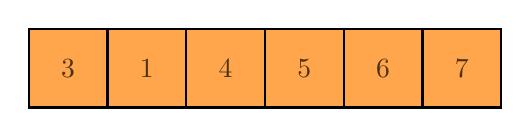
\begin{tikzpicture}
	\node (rect) at (0,0) [draw, thick, fill=orange, fill opacity=0.7,
		minimum width=1cm,minimum height=1cm] {$3$};
	\node (rect) at (1,0) [draw, thick, fill=orange, fill opacity=0.7,
		minimum width=1cm,minimum height=1cm] {$1$};
	\node (rect) at (2,0) [draw, thick, fill=orange, fill opacity=0.7,
		minimum width=1cm,minimum height=1cm] {$4$};
	\node (rect) at (3,0) [draw, thick, fill=orange, fill opacity=0.7,
		minimum width=1cm,minimum height=1cm] {$5$};
	\node (rect) at (4,0) [draw, thick, fill=orange, fill opacity=0.7,
		minimum width=1cm,minimum height=1cm] {$6$};
	\node (rect) at (5,0) [draw, thick, fill=orange, fill opacity=0.7,
		minimum width=1cm,minimum height=1cm] {$7$};
\end{tikzpicture}

这是一个数组:[3,1,4,5,6,7],它本质上就是在一段连续的内存片段上存储的一串数据,由于int占了四个字节,所以每一个数组元素的地址相差四位。

接下来分析数组中常见的操作的算法复杂度:
\begin{itemize}
	\item Lookup O(1) 根据索引去查找元素,由于数组中可以通过中括号访问符进行访问,所以不论访问哪一个元素,算法复杂度均为O(1)
	\item Insert O(n) 进行元素插入,如果在末尾进行元素插入,算法复杂度为O(1),但是如果在第一位插入,我们就需要将每一位都往后挪动一位,所以复杂度为O(n),通常我们都考虑最坏的情况,所以算法复杂度为O(n)
	\item Delete O(n) 无论删除哪一个元素,其他元素都需要往前移动一位,所以最终算法复杂度为O(n)
\end{itemize}
\section{Practice: To create an Array Class with Java}

\begin{example}
	在Java中,创建一个MikeArray类型,要求要满足以下几点,1.具有insert方法,可以在数组末尾插入元素,2.具有removeAt(int index)方法,在index处删除对应的元素,3.实现print方法,打印出数组中所有的元素 4. indexOf方法,返回目标元素第一次出现在数组中的索引,如果没有出现元素,则返回索引-1,4.动态扩充,在使用insert方法的时候如果超出了数组本身的长度,扩容到原数组容量的2倍,5.构造方法是给出数组的长度length进行数组构造的。
\end{example}
\begin{minted}[]{java}
public class MArray {
    private int[]items;
    private int count=0;
    public MArray(int length){
        items=new int[length];
    }

    public void print(){
        for(int i=0;i<count;i++){
            System.out.println(items[i]);
        }
    }

    public void insert(int element){
        //if the array is full
        if(items.length==count){
            //Create a new array (twice the size)
            int array[]=new int[count*2];
            //Copy all the items into new Array
            for(int i=0;i<count;i++){
                array[i]=items[i];
            }
            //set the items to the new array
            items=array;
        }
        items[count++]=element;
    }



}

\end{minted}

\begin{minted}[]{java}
	    public void removeAt(int index){
            if(index<0||index>=count){
               throw new IllegalArgumentException();
            }
            else{
                //[10,20,30,40]
                // index:1
                for(int i=index;i<count;i++){
                items[i]=items[i+1];
                }
                count--;
            }
    }

    public int indexOf(int item){
        //获取元素的位置
        //肯定是有可能遍历完整个都没有存在的
        for(int i=0;i<count;i++){
            if(items[i]==item){
                return i;
            }

        }
        return -1;
    }
\end{minted}

\part{Part One Title}

%----------------------------------------------------------------------------------------
%	SECTIONING EXAMPLES CHAPTER
%----------------------------------------------------------------------------------------

\chapterimage{orange2.jpg} % Chapter heading image
\chapterspaceabove{6.75cm} % Whitespace from the top of the page to the chapter title on chapter pages
\chapterspacebelow{7.25cm} % Amount of vertical whitespace from the top margin to the start of the text on chapter pages

%------------------------------------------------

\chapter{Sectioning Examples}\index{Sectioning}

\section{Section Title}\index{Sectioning!Sections}

Lorem ipsum dolor sit amet, consectetur adipiscing elit\footnote{Footnote example text\ldots Lorem ipsum dolor sit amet, consectetur adipiscing elit. Praesent porttitor arcu luctus, imperdiet urna iaculis, mattis eros. Pellentesque iaculis odio vel nisl ullamcorper, nec faucibus ipsum molestie.}. Praesent porttitor arcu luctus, imperdiet urna iaculis, mattis eros. Pellentesque iaculis odio vel nisl ullamcorper, nec faucibus ipsum molestie. Sed dictum nisl non aliquet porttitor. Etiam vulputate arcu dignissim, finibus sem et, viverra nisl. Aenean luctus congue massa, ut laoreet metus ornare in. Nunc fermentum nisi imperdiet lectus tincidunt vestibulum at ac elit. Nulla mattis nisl eu malesuada suscipit.

Aliquam arcu turpis, ultrices sed luctus ac, vehicula id metus. Morbi eu feugiat velit, et tempus augue. Proin ac mattis tortor. Donec tincidunt, ante rhoncus luctus semper, arcu lorem lobortis justo, nec convallis ante quam quis lectus. Aenean tincidunt sodales massa, et hendrerit tellus mattis ac. Sed non pretium nibh. Donec cursus maximus luctus. Vivamus lobortis eros et massa porta porttitor.

\subsection{Subsection Title}\index{Sectioning!Subsections}

Fusce varius orci ac magna dapibus porttitor. In tempor leo a neque bibendum sollicitudin. Nulla pretium fermentum nisi, eget sodales magna facilisis eu. Praesent aliquet nulla ut bibendum lacinia. Donec vel mauris vulputate, commodo ligula ut, egestas orci. Suspendisse commodo odio sed hendrerit lobortis. Donec finibus eros erat, vel ornare enim mattis et. Donec finibus dolor quis dolor tempus consequat. Mauris fringilla dui id libero egestas, ut mattis neque ornare. Ut condimentum urna pharetra ipsum consequat, eu interdum elit cursus. Vivamus scelerisque tortor et nunc ultricies, id tincidunt libero pharetra. Aliquam eu imperdiet leo. Morbi a massa volutpat velit condimentum convallis et facilisis dolor.

In hac habitasse platea dictumst. Curabitur mattis elit sit amet justo luctus vestibulum. In hac habitasse platea dictumst. Pellentesque lobortis justo enim, a condimentum massa tempor eu. Ut quis nulla a quam pretium eleifend nec eu nisl. Nam cursus porttitor eros, sed luctus ligula convallis quis. Nam convallis, ligula in auctor euismod, ligula mauris fringilla tellus, et egestas mauris odio eget diam. Praesent sodales in ipsum eu dictum. Mauris interdum porttitor fringilla. Proin tincidunt sodales leo at ornare. Donec tempus magna non mauris gravida luctus. Cras vitae arcu vitae mauris eleifend scelerisque. Nam sem sapien, vulputate nec felis eu, blandit convallis risus. Pellentesque sollicitudin venenatis tincidunt. In et ipsum libero.

\subsubsection{Subsubsection Title} \index{Sectioning!Subsubsections}

Maecenas consectetur metus at tellus finibus condimentum. Proin arcu lectus, ultrices non tincidunt et, tincidunt ut quam. Integer luctus posuere est, non maximus ante dignissim quis. Nunc a cursus erat. Curabitur suscipit nibh in tincidunt sagittis. Nam malesuada vestibulum quam id gravida. Proin ut dapibus velit. Vestibulum eget quam quis ipsum semper convallis. Duis consectetur nibh ac diam dignissim, id condimentum enim dictum. Nam aliquet ligula eu magna pellentesque, nec sagittis leo lobortis. Aenean tincidunt dignissim egestas. Morbi efficitur risus ante, id tincidunt odio pulvinar vitae.

\paragraph{Paragraph Title}\index{Sectioning!Paragraphs} Nullam mollis tellus lorem, sed congue ipsum euismod a. Donec pulvinar neque sed ligula ornare sodales. Nulla sagittis vel lectus nec laoreet. Nulla volutpat malesuada turpis at ultricies. Ut luctus velit odio, sagittis volutpat erat aliquet vel. Donec ac neque eget neque volutpat mollis. Vestibulum viverra ligula et sapien bibendum, vel vulputate ex euismod. Curabitur nec velit velit. Aliquam vulputate lorem elit, id tempus nisl finibus sit amet. Curabitur ex turpis, consequat at lectus id, imperdiet molestie augue. Curabitur eu eros molestie purus commodo hendrerit. Quisque auctor ipsum nec mauris malesuada, non fringilla nibh viverra. Quisque gravida, metus quis semper pulvinar, dolor nisl suscipit leo, vestibulum volutpat ante justo ultrices diam. Sed id facilisis turpis, et aliquet eros.

In malesuada ullamcorper urna, sed dapibus diam sollicitudin non. Donec elit odio, accumsan ac nisl a, tempor imperdiet eros. Donec porta tortor eu risus consequat, a pharetra tortor tristique. Morbi sit amet laoreet erat. Morbi et luctus diam, quis porta ipsum. Quisque libero dolor, suscipit id facilisis eget, sodales volutpat dolor. Nullam vulputate interdum aliquam. Mauris id convallis erat, ut vehicula neque. Sed auctor nibh et elit fringilla, nec ultricies dui sollicitudin. Vestibulum vestibulum luctus metus venenatis facilisis. Suspendisse iaculis augue at vehicula ornare. Sed vel eros ut velit fermentum porttitor sed sed massa. Fusce venenatis, metus a rutrum sagittis, enim ex maximus velit, id semper nisi velit eu purus.

%------------------------------------------------

\section*{Unnumbered Section}

\subsection*{Unnumbered Subsection}

\subsubsection*{Unnumbered Subsubsection}

%----------------------------------------------------------------------------------------
%	IN-TEXT ELEMENT EXAMPLES CHAPTER
%----------------------------------------------------------------------------------------

\chapter{In-text Element Examples}

\section{Referencing Publications}\index{Citation}

This statement requires citation \cite{Smith:2022jd}; this one is more specific \cite[162]{Smith:2021qr}.

%------------------------------------------------

\section{Link Examples}\index{Links}

This is a URL link: \href{https://www.latextemplates.com}{LaTeX Templates}. This is an email link: \href{mailto:example@example.com}{example@example.com}. This is a monospaced URL link: \url{https://www.LaTeXTemplates.com}.

%------------------------------------------------

\section{Lists}\index{Lists}

Lists are useful to present information in a concise and/or ordered way.

\subsection{Numbered List}\index{Lists!Numbered List}

\begin{enumerate}
	\item First numbered item
	      \begin{enumerate}
		      \item First indented numbered item
		      \item Second indented numbered item
		            \begin{enumerate}
			            \item First second-level indented numbered item
		            \end{enumerate}
	      \end{enumerate}
	\item Second numbered item
	\item Third numbered item
\end{enumerate}

\subsection{Bullet Point List}\index{Lists!Bullet Points}

\begin{itemize}
	\item First bullet point item
	      \begin{itemize}
		      \item First indented bullet point item
		      \item Second indented bullet point item
		            \begin{itemize}
			            \item First second-level indented bullet point item
		            \end{itemize}
	      \end{itemize}
	\item Second bullet point item
	\item Third bullet point item
\end{itemize}

\subsection{Descriptions and Definitions}\index{Lists!Descriptions and Definitions}

\begin{description}
	\item[Name] Description
	\item[Word] Definition
	\item[Comment] Elaboration
\end{description}

%------------------------------------------------

\section{International Support}

àáâäãåèéêëìíîïòóôöõøùúûüÿýñçčšž

\noindent ÀÁÂÄÃÅÈÉÊËÌÍÎÏÒÓÔÖÕØÙÚÛÜŸÝÑ

\noindent ßÇŒÆČŠŽ

%------------------------------------------------

\section{Ligatures}

fi fj fl ffl ffi Ty

%----------------------------------------------------------------------------------------
%	PART
%----------------------------------------------------------------------------------------

\part{Part Two Title}

%----------------------------------------------------------------------------------------
%	MATHEMATICS EXAMPLES CHAPTER
%----------------------------------------------------------------------------------------

\chapter{Mathematics}

\section{Theorems}\index{Theorems}

\subsection{Several equations}\index{Theorems!Several Equations}

This is a theorem consisting of several equations.

\begin{theorem}[Name of the theorem] % Specify a name/title in square brackets, or leave them out for no title
	In $E=\mathbb{R}^n$ all norms are equivalent. It has the properties:
	\begin{align}
		 & \big| ||\mathbf{x}|| - ||\mathbf{y}|| \big|\leq || \mathbf{x}- \mathbf{y}||                            \\
		 & ||\sum_{i=1}^n\mathbf{x}_i||\leq \sum_{i=1}^n||\mathbf{x}_i||\quad\text{where $n$ is a finite integer}
	\end{align}
\end{theorem}

\subsection{Single Line}\index{Theorems!Single Line}

This is a theorem consisting of just one line.

\begin{theorem} % Specify a name/title in square brackets, or leave them out for no title
	A set $\mathcal{D}(G)$ in dense in $L^2(G)$, $|\cdot|_0$.
\end{theorem}

%------------------------------------------------

\section{Definitions}\index{Definitions}

A definition can be mathematical or it could define a concept.

\begin{definition}[Definition name] % Specify a name/title in square brackets, or leave them out for no title
	Given a vector space $E$, a norm on $E$ is an application, denoted $||\cdot||$, $E$ in $\mathbb{R}^+=[0,+\infty[$ such that:
	\begin{align}
		 & ||\mathbf{x}||=0\ \Rightarrow\ \mathbf{x}=\mathbf{0}        \\
		 & ||\lambda \mathbf{x}||=|\lambda|\cdot ||\mathbf{x}||        \\
		 & ||\mathbf{x}+\mathbf{y}||\leq ||\mathbf{x}||+||\mathbf{y}||
	\end{align}
\end{definition}

%------------------------------------------------

\section{Notations}\index{Notations}

\begin{notation} % Specify a name/title in square brackets, or leave them out for no title
	Given an open subset $G$ of $\mathbb{R}^n$, the set of functions $\varphi$ are:
	\begin{enumerate}
		\item Bounded support $G$;
		\item Infinitely differentiable;
	\end{enumerate}
	a vector space is denoted by $\mathcal{D}(G)$.
\end{notation}

%------------------------------------------------

\section{Remarks}\index{Remarks}

This is an example of a remark.

\begin{remark}
	The concepts presented here are now in conventional employment in mathematics. Vector spaces are taken over the field $\mathbb{K}=\mathbb{R}$, however, established properties are easily extended to $\mathbb{K}=\mathbb{C}$.
\end{remark}

%------------------------------------------------

\section{Corollaries}\index{Corollaries}

\begin{corollary}[Corollary name] % Specify a name/title in square brackets, or leave them out for no title
	The concepts presented here are now in conventional employment in mathematics. Vector spaces are taken over the field $\mathbb{K}=\mathbb{R}$, however, established properties are easily extended to $\mathbb{K}=\mathbb{C}$.
\end{corollary}

%------------------------------------------------

\section{Propositions}\index{Propositions}

\subsection{Several equations}\index{Propositions!Several Equations}

\begin{proposition}[Proposition name] % Specify a name/title in square brackets, or leave them out for no title
	It has the properties:
	\begin{align}
		 & \big| ||\mathbf{x}|| - ||\mathbf{y}|| \big|\leq || \mathbf{x}- \mathbf{y}||                            \\
		 & ||\sum_{i=1}^n\mathbf{x}_i||\leq \sum_{i=1}^n||\mathbf{x}_i||\quad\text{where $n$ is a finite integer}
	\end{align}
\end{proposition}

\subsection{Single Line}\index{Propositions!Single Line}

\begin{proposition} % Specify a name/title in square brackets, or leave them out for no title
	Let $f,g\in L^2(G)$; if $\forall \varphi\in\mathcal{D}(G)$, $(f,\varphi)_0=(g,\varphi)_0$ then $f = g$.
\end{proposition}

%------------------------------------------------

\section{Examples}\index{Examples}

\subsection{Equation Example}\index{Examples!Equation}

\begin{example} % Specify a name/title in square brackets, or leave them out for no title
	Let $G=\{x\in\mathbb{R}^2:|x|<3\}$ and denoted by: $x^0=(1,1)$; consider the function:
	\begin{equation}
		f(x)=\left\{\begin{aligned}                                                                                     & \mathrm{e}^{|x|} &  & \text{si $|x-x^0|\leq 1/2$} \\
                                                                                                    & 0                &  & \text{si $|x-x^0|> 1/2$}\end{aligned}\right.
	\end{equation}
	The function $f$ has bounded support, we can take $A=\{x\in\mathbb{R}^2:|x-x^0|\leq 1/2+\epsilon\}$ for all $\epsilon\in\mathopen{]}0\,;5/2-\sqrt{2}\mathclose{[}$.
\end{example}

\subsection{Text Example}\index{Examples!Text}

\begin{example}[Example name] % Specify a name/title in square brackets, or leave them out for no title
	Aliquam arcu turpis, ultrices sed luctus ac, vehicula id metus. Morbi eu feugiat velit, et tempus augue. Proin ac mattis tortor. Donec tincidunt, ante rhoncus luctus semper, arcu lorem lobortis justo, nec convallis ante quam quis lectus. Aenean tincidunt sodales massa, et hendrerit tellus mattis ac. Sed non pretium nibh. Donec cursus maximus luctus. Vivamus lobortis eros et massa porta porttitor.
\end{example}

%------------------------------------------------

\section{Exercises}\index{Exercises}

\begin{exercise} % Specify a name/title in square brackets, or leave them out for no title
	This is a good place to ask a question to test learning progress or further cement ideas into students' minds.
\end{exercise}

%------------------------------------------------

\section{Problems}\index{Problems}

\begin{problem} % Specify a name/title in square brackets, or leave them out for no title
What is the average airspeed velocity of an unladen swallow?
\end{problem}

%------------------------------------------------

\section{Vocabulary}\index{Vocabulary}

Define a word to improve a students' vocabulary.

\begin{vocabulary}[Word] % Specify a name/title in square brackets, or leave them out for no title
	Definition of word.
\end{vocabulary}

%----------------------------------------------------------------------------------------
%	PRESENTING INFORMATION/RESULTS EXAMPLES CHAPTER
%----------------------------------------------------------------------------------------

\chapterimage{orange3.jpg} % Chapter heading image
\chapterspaceabove{6.25cm} % Whitespace from the top of the page to the chapter title on chapter pages
\chapterspacebelow{7.5cm} % Amount of vertical whitespace from the top margin to the start of the text on chapter pages

%------------------------------------------------

\chapter{Presenting Information and Results with a Long Chapter Title}

\section{Table}\index{Table}

Lorem ipsum dolor sit amet, consectetur adipiscing elit. Praesent porttitor arcu luctus, imperdiet urna iaculis, mattis eros. Pellentesque iaculis odio vel nisl ullamcorper, nec faucibus ipsum molestie. Sed dictum nisl non aliquet porttitor. Etiam vulputate arcu dignissim, finibus sem et, viverra nisl. Aenean luctus congue massa, ut laoreet metus ornare in. Nunc fermentum nisi imperdiet lectus tincidunt vestibulum at ac elit. Nulla mattis nisl eu malesuada suscipit.

\begin{table}[H] % Use [H] to suppress floating and place the figure/table exactly where it is specified in the text
	\centering % Horizontally center the table on the page
	\begin{tabular}{L{0.15\textwidth} R{0.15\textwidth} R{0.15\textwidth}} % Specify column alignment with L{width}, C{width} and R{width} for fixed-width columns, or the default latex l, c and r for flexible-width columns
		\toprule
		\textbf{Treatments} & \textbf{Response 1} & \textbf{Response 2} \\
		\midrule
		Treatment 1         & 0.0003262           & 0.562               \\
		Treatment 2         & 0.0015681           & 0.910               \\
		Treatment 3         & 0.0009271           & 0.296               \\
		\bottomrule
	\end{tabular}
	\caption{Table caption.}
	\label{tab:example} % Unique label used for referencing the table in-text
\end{table}

Referencing \autoref{tab:example} in-text using its label.

\begin{table}[t] % Floating table, [t] tells LaTeX to place it at the top of the next available page
	\centering % Horizontally center the table on the page
	\begin{tabular}{L{0.15\textwidth} R{0.15\textwidth} R{0.15\textwidth}} % Specify column alignment with L{width}, C{width} and R{width} for fixed-width columns, or the default latex l, c and r for flexible-width columns
		\toprule
		\textbf{Treatments} & \textbf{Response 1} & \textbf{Response 2} \\
		\midrule
		Treatment 1         & 0.0003262           & 0.562               \\
		Treatment 2         & 0.0015681           & 0.910               \\
		Treatment 3         & 0.0009271           & 0.296               \\
		\bottomrule
	\end{tabular}
	\caption{Floating table.}
	\label{tab:floating} % Unique label used for referencing the table in-text
\end{table}

%------------------------------------------------

\section{Figure}\index{Figure}

Lorem ipsum dolor sit amet, consectetur adipiscing elit. Praesent porttitor arcu luctus, imperdiet urna iaculis, mattis eros. Pellentesque iaculis odio vel nisl ullamcorper, nec faucibus ipsum molestie. Sed dictum nisl non aliquet porttitor. Etiam vulputate arcu dignissim, finibus sem et, viverra nisl. Aenean luctus congue massa, ut laoreet metus ornare in. Nunc fermentum nisi imperdiet lectus tincidunt vestibulum at ac elit. Nulla mattis nisl eu malesuada suscipit.

\begin{figure}[H] % Use [H] to suppress floating and place the figure/table exactly where it is specified in the text
	\centering % Horizontally center the figure on the page
	
\includegraphics[width=0.5\textwidth]{creodocs_logo.pdf} % Include the figure image
	\caption{Figure caption.}
	\label{fig:placeholder} % Unique label used for referencing the figure in-text
\end{figure}

Referencing \autoref{fig:placeholder} in-text using its label.

\begin{figure}[b] % Floating figure, [b] tells LaTeX to place it at the bottom of the next available page
	\centering % Horizontally center the figure on the page
	
\includegraphics[width=\textwidth]{creodocs_logo.pdf} % Include the figure image
	\caption{Floating figure.}
	\label{fig:floating} % Unique label used for referencing the figure in-text
\end{figure}

%----------------------------------------------------------------------------------------

\stopcontents[part] % Manually stop the 'part' table of contents here so the previous Part page table of contents doesn't list the following chapters

%----------------------------------------------------------------------------------------
%	BIBLIOGRAPHY
%----------------------------------------------------------------------------------------

\chapterimage{} % Chapter heading image
\chapterspaceabove{2.5cm} % Whitespace from the top of the page to the chapter title on chapter pages
\chapterspacebelow{2cm} % Amount of vertical whitespace from the top margin to the start of the text on chapter pages

%------------------------------------------------

\chapter*{Bibliography}
\markboth{\sffamily\normalsize\bfseries Bibliography}{\sffamily\normalsize\bfseries Bibliography} % Set the page headers to display a Bibliography chapter name
\addcontentsline{toc}{chapter}{\textcolor{ocre}{Bibliography}} % Add a Bibliography heading to the table of contents

\section*{Articles}
\addcontentsline{toc}{section}{Articles} % Add the Articles subheading to the table of contents

\printbibliography[heading=bibempty, type=article] % Output article bibliography entries

\section*{Books}
\addcontentsline{toc}{section}{Books} % Add the Books subheading to the table of contents

\printbibliography[heading=bibempty, type=book] % Output book bibliography entries

%----------------------------------------------------------------------------------------
%	INDEX
%----------------------------------------------------------------------------------------

\cleardoublepage % Make sure the index starts on an odd (right side) page
\phantomsection
\addcontentsline{toc}{chapter}{\textcolor{ocre}{Index}} % Add an Index heading to the table of contents
\printindex % Output the index

%----------------------------------------------------------------------------------------
%	APPENDICES
%----------------------------------------------------------------------------------------

\chapterimage{orange2.jpg} % Chapter heading image
\chapterspaceabove{6.75cm} % Whitespace from the top of the page to the chapter title on chapter pages
\chapterspacebelow{7.25cm} % Amount of vertical whitespace from the top margin to the start of the text on chapter pages

\begin{appendices}

	\renewcommand{\chaptername}{Appendix} % Change the chapter name to Appendix, i.e. "Appendix A: Title", instead of "Chapter A: Title" in the headers

	%------------------------------------------------

	\chapter{Appendix Chapter Title}

	\section{Appendix Section Title}

	Lorem ipsum dolor sit amet, consectetur adipiscing elit. Aliquam auctor mi risus, quis tempor libero hendrerit at. Duis hendrerit placerat quam et semper. Nam ultricies metus vehicula arcu viverra, vel ullamcorper justo elementum. Pellentesque vel mi ac lectus cursus posuere et nec ex. Fusce quis mauris egestas lacus commodo venenatis. Ut at arcu lectus. Donec et urna nunc. Morbi eu nisl cursus sapien eleifend tincidunt quis quis est. Donec ut orci ex. Praesent ligula enim, ullamcorper non lorem a, ultrices volutpat dolor. Nullam at imperdiet urna. Pellentesque nec velit eget est euismod pretium.

	%------------------------------------------------

	\chapter{Appendix Chapter Title}

	\section{Appendix Section Title}

	Lorem ipsum dolor sit amet, consectetur adipiscing elit. Aliquam auctor mi risus, quis tempor libero hendrerit at. Duis hendrerit placerat quam et semper. Nam ultricies metus vehicula arcu viverra, vel ullamcorper justo elementum. Pellentesque vel mi ac lectus cursus posuere et nec ex. Fusce quis mauris egestas lacus commodo venenatis. Ut at arcu lectus. Donec et urna nunc. Morbi eu nisl cursus sapien eleifend tincidunt quis quis est. Donec ut orci ex. Praesent ligula enim, ullamcorper non lorem a, ultrices volutpat dolor. Nullam at imperdiet urna. Pellentesque nec velit eget est euismod pretium.

	%------------------------------------------------

\end{appendices}

%----------------------------------------------------------------------------------------

\end{document}
